% !TeX spellcheck = sk_SK-Slovak
\documentclass[a4paper]{article}
\usepackage[slovak]{babel}
\usepackage[utf8]{inputenc}
\usepackage[T1]{fontenc}
\usepackage{a4wide}
\usepackage{amsmath}
\usepackage{amsfonts}
\usepackage{amsthm,amssymb}
\usepackage{mathrsfs}
\usepackage[small,bf]{caption}
\usepackage{subcaption}
\usepackage{xcolor}
\usepackage{graphicx}
\usepackage{enumerate}
\usepackage{hyperref}
\usepackage[a4paper, total={7in, 10.2in}]{geometry}



\pagestyle{empty}
\setlength{\parindent}{0pt}

\newenvironment{modenumerate}
{\enumerate\setupmodenumerate}
{\endenumerate}

%\renewcommand{\thesubsection}{\thesection.\alph{subsection}}
\renewcommand{\thesubsection}{\alph{subsection})}


\begin{document} 
	
	\pagenumbering{arabic}
	\pagestyle{plain}
	
	\begin{center}
		\sc\large
		PHYSICAL BASED ANIMATIONS AND MATHEMATICAL MODELING HW 2 
		\\
		Matica hybnosti
	\end{center}

	Autor: Marián Kravec
	\\
	\\
	Našou úlohou je vypočítať hmotnosť, tensor zotrvačnosti a ťažisko následujúceho telesa:
	
	\centerline{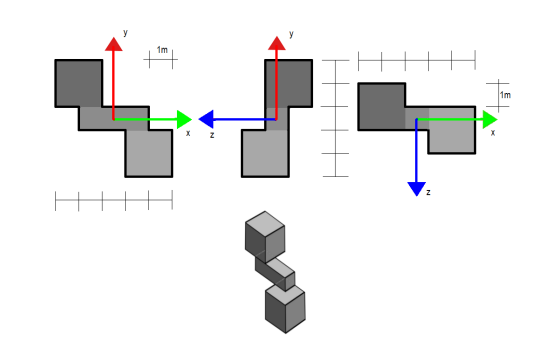
\includegraphics[width=0.7\textwidth]{podorysy}} 
	
	Prvá vec čo si môžeme všimnúť je, že aj napriek tomu, že naše teleso vyzerá pomerne komplikovane vieme ho rozdeliť na trojicu hranolov z ktorých dve hranoly sú dokonca kocky.
	\\
	\\
	To nám úlohu zjednodušuje keďže vieme, že pre hranol sa matica zotrvačnosti vypočíta následovne:
	\begin{align*}
		J_0 = \begin{bmatrix}
			\frac{m}{12}(h^2 + d^2) & 0 & 0 \\
			0 & \frac{m}{12}(w^2 + d^2) & 0 \\
			0 & 0 & \frac{m}{12}(w^2 + h^2)
		\end{bmatrix}
	\end{align*}
	Kde $(w, h, d)$ sú rozmery hranolu a $m$ je jeho hmotnosť. Avšak tento vzorec platí iba ak os otáčania prechádza ťažiskom daného hranolu. Ak je tento hranol posunutý v súradnicovej sústave o vektor $\boldsymbol{r}$ tak jeho maticu hybnosti vieme vypočítať následovne:
	\begin{align*}
		J = J_0 + m(r^TrI-rr^T)
	\end{align*}
	Poďme si teraz vypočítať rozmery jednotlivých našich rozmerov. Ak sa nemýlim v zadaní nie je ich poloha a rozmery určené presnejšie ako z pohľadu na ich vizualizáciu čiže pôdorysy. Z pôdorysov vidíme, že všetky 3 hranoly majú všetky hrany rovnobežné s niektorou zo štandardných osí čo uľahčuje určovanie ich rozmerov.
	\\
	\\
	Začnime s kockou ktorá je na pôdorysoch zobrazená ako najtmavšia. Vidíme, že tento hranol má všetky rozmery 2 metre, ak budeme považovať meter za základnú jednotku nášho priestoru tak rozmery vieme zapísať ako $(w, h, d) = (2, 2, 2)$. 
	\\
	\\
	Ak sa pozrieme na kocku na opačnej strana telesa (najsvetlejšia) vidíme, že jej rozmery sú totožné čiže takisto ju vieme zapísať $(w, h, d) = (2, 2, 2)$.
	\\
	\\
	Nakoniec nám zostal hranol v strede. 
\end{document}
